In this section the conformation of FAK in absence of \pip{} and other FAK molecules is analyzed. For this purpose the simulation data of setup 1 is used.\\
\\
First the COM distances of F1 to the N-lobe ($d_\text{F1-N}$) and F2 to the C-lobe ($d_\text{F2-C}$) are considered. In \autoref{free:f2clf1nl} a hexagonal binning plot of both values can be found, which indicates, that there are two different states. Spot 1 shows large values of $3.8\,\si{\nano\metre}$ for $d_\text{F2-C}$, while $d_\text{F1-N} \approx 3.5\,\si{\nano\metre}$. In contrast to this the values of $d_\text{F2-C}$ are much smaller in spot 2 and $d_\text{F1-N}$ gets larger. Certainly these spots can not be seen in the contact area of the interface (see \autoref{mem:contactarea}), which is symmetrically distributed around $27.5\,\si{\nano\metre}^2$.
%
%
%
\begin{figure}
	\centering
	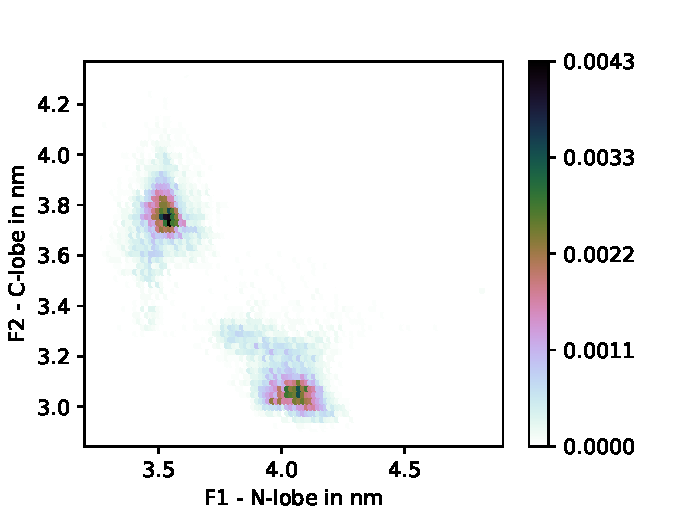
\includegraphics[width=.7\textwidth]{figures/results/free_f1f2}
	\captionof{figure}{Two dimensional histogram of $d_\text{F1-N}$ and $d_\text{F2-C}$. The histogram is normed and the color indicates the relative frequency.}
	\label{free:f2clf1nl}
\end{figure}
%
%
%
A contact map of the interface between the FERM domain and the kinase for frames of spot 2 can be found in \autoref{free:contact}. Two contact areas can be identified at the interface. The first one (area 1) is located between F1 and the N-lobe/activation loop. It shows i.e. contacts between \acid{Y}{576} and \acid{Y}{577} and residues of the FERM domain. The minimal distance in this area, between residue \acid{H}{41} and \acid{Y}{576}, is $0.45\,\si{\nano\metre}$ with an RMSF value of $0.03\,\si{\nano\metre}$. This reflects the burying of the activity regulating residues in closed state.\\
The second contact area (area 2) is located between F2 and the C-lobe. The spots occur around the residues \acid{Y}{180} and \acid{D}{200} of F2 as well as \acid{F}{596} and \acid{R}{665}. The minimal distance in this area occurs between \acid{Y}{180} and \acid{F}{596} with $0.45\,\si{\nano\metre}$ and an RMSF value of $0.02\,\si{\nano\metre}$. These two residues have been reported as important actors in the interface, because a mutation disturbs the interface and enhances the activation of FAK.\\
The linker show contacts with both domains. Interestingly the minimal distance in the marked areas (area 3 and area 4) occur between the autophosphorylation site \acid{Y}{397} and \acid{H}{58} ($0.45\,\si{\nano\metre}$, RMSF $0.03\,\si{\nano\metre}$) in F1 as well as \acid{Y}{576} ($0.50\,\si{\nano\metre}$, RMSF $0.10\,\si{\nano\metre}$) in the kinase. This is consistent with the concept, that autophosphorylation is prevented in closed conformation by a binding of the linker to the FERM domain.
%
%
%
\begin{figure}
	\centering
	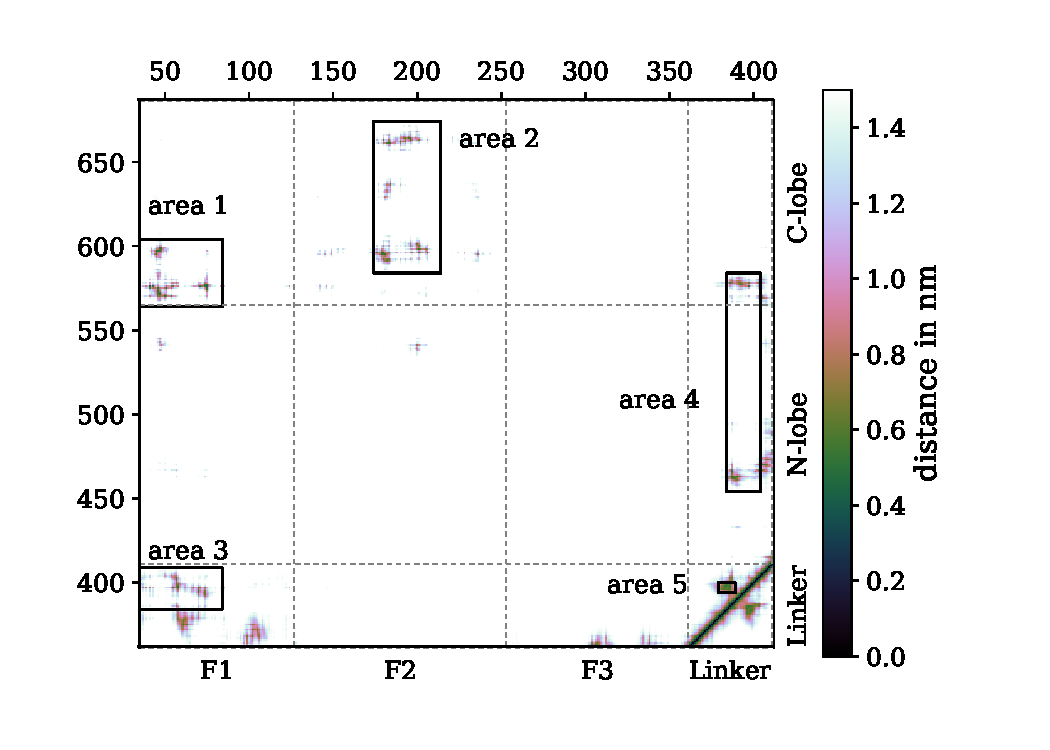
\includegraphics[width=.7\textwidth]{figures/results/contactmap_free}
	\captionof{figure}{Contactmap of interface between FERM domain and kinase}
	\label{free:contact}
\end{figure}
%
%
%
In contrast to \autoref{free:contact}, the contact map for frames of spot 1 show less contacts between F2 and the C-lobe, i.e. around the mentioned residues \acid{Y}{180} to \acid{M}{183}. A few additional contacts appear between F1 and the N-lobe, but these are only minor spots.